\documentclass[1p]{elsarticle_modified}
%\bibliographystyle{elsarticle-num}

%\usepackage[colorlinks]{hyperref}
%\usepackage{abbrmath_seonhwa} %\Abb, \Ascr, \Acal ,\Abf, \Afrak
\usepackage{amsfonts}
\usepackage{amssymb}
\usepackage{amsmath}
\usepackage{amsthm}
\usepackage{scalefnt}
\usepackage{amsbsy}
\usepackage{kotex}
\usepackage{caption}
\usepackage{subfig}
\usepackage{color}
\usepackage{graphicx}
\usepackage{xcolor} %% white, black, red, green, blue, cyan, magenta, yellow
\usepackage{float}
\usepackage{setspace}
\usepackage{hyperref}

\usepackage{tikz}
\usetikzlibrary{arrows}

\usepackage{multirow}
\usepackage{array} % fixed length table
\usepackage{hhline}

%%%%%%%%%%%%%%%%%%%%%
\makeatletter
\renewcommand*\env@matrix[1][\arraystretch]{%
	\edef\arraystretch{#1}%
	\hskip -\arraycolsep
	\let\@ifnextchar\new@ifnextchar
	\array{*\c@MaxMatrixCols c}}
\makeatother %https://tex.stackexchange.com/questions/14071/how-can-i-increase-the-line-spacing-in-a-matrix
%%%%%%%%%%%%%%%

\usepackage[normalem]{ulem}

\newcommand{\msout}[1]{\ifmmode\text{\sout{\ensuremath{#1}}}\else\sout{#1}\fi}
%SOURCE: \msout is \stkout macro in https://tex.stackexchange.com/questions/20609/strikeout-in-math-mode

\newcommand{\cancel}[1]{
	\ifmmode
	{\color{red}\msout{#1}}
	\else
	{\color{red}\sout{#1}}
	\fi
}

\newcommand{\add}[1]{
	{\color{blue}\uwave{#1}}
}

\newcommand{\replace}[2]{
	\ifmmode
	{\color{red}\msout{#1}}{\color{blue}\uwave{#2}}
	\else
	{\color{red}\sout{#1}}{\color{blue}\uwave{#2}}
	\fi
}

\newcommand{\Sol}{\mathcal{S}} %segment
\newcommand{\D}{D} %diagram
\newcommand{\A}{\mathcal{A}} %arc


%%%%%%%%%%%%%%%%%%%%%%%%%%%%%5 test

\def\sl{\operatorname{\textup{SL}}(2,\Cbb)}
\def\psl{\operatorname{\textup{PSL}}(2,\Cbb)}
\def\quan{\mkern 1mu \triangleright \mkern 1mu}

\theoremstyle{definition}
\newtheorem{thm}{Theorem}[section]
\newtheorem{prop}[thm]{Proposition}
\newtheorem{lem}[thm]{Lemma}
\newtheorem{ques}[thm]{Question}
\newtheorem{cor}[thm]{Corollary}
\newtheorem{defn}[thm]{Definition}
\newtheorem{exam}[thm]{Example}
\newtheorem{rmk}[thm]{Remark}
\newtheorem{alg}[thm]{Algorithm}

\newcommand{\I}{\sqrt{-1}}
\begin{document}

%\begin{frontmatter}
%
%\title{Boundary parabolic representations of knots up to 8 crossings}
%
%%% Group authors per affiliation:
%\author{Yunhi Cho} 
%\address{Department of Mathematics, University of Seoul, Seoul, Korea}
%\ead{yhcho@uos.ac.kr}
%
%
%\author{Seonhwa Kim} %\fnref{s_kim}}
%\address{Center for Geometry and Physics, Institute for Basic Science, Pohang, 37673, Korea}
%\ead{ryeona17@ibs.re.kr}
%
%\author{Hyuk Kim}
%\address{Department of Mathematical Sciences, Seoul National University, Seoul 08826, Korea}
%\ead{hyukkim@snu.ac.kr}
%
%\author{Seokbeom Yoon}
%\address{Department of Mathematical Sciences, Seoul National University, Seoul, 08826,  Korea}
%\ead{sbyoon15@snu.ac.kr}
%
%\begin{abstract}
%We find all boundary parabolic representation of knots up to 8 crossings.
%
%\end{abstract}
%\begin{keyword}
%    \MSC[2010] 57M25 
%\end{keyword}
%
%\end{frontmatter}

%\linenumbers
%\tableofcontents
%
\newcommand\colored[1]{\textcolor{white}{\rule[-0.35ex]{0.8em}{1.4ex}}\kern-0.8em\color{red} #1}%
%\newcommand\colored[1]{\textcolor{white}{ #1}\kern-2.17ex	\textcolor{white}{ #1}\kern-1.81ex	\textcolor{white}{ #1}\kern-2.15ex\color{red}#1	}

{\Large $\underline{12n_{0430}~(K12n_{0430})}$}

\setlength{\tabcolsep}{10pt}
\renewcommand{\arraystretch}{1.6}
\vspace{1cm}\begin{tabular}{m{100pt}>{\centering\arraybackslash}m{274pt}}
\multirow{5}{120pt}{
	\centering
	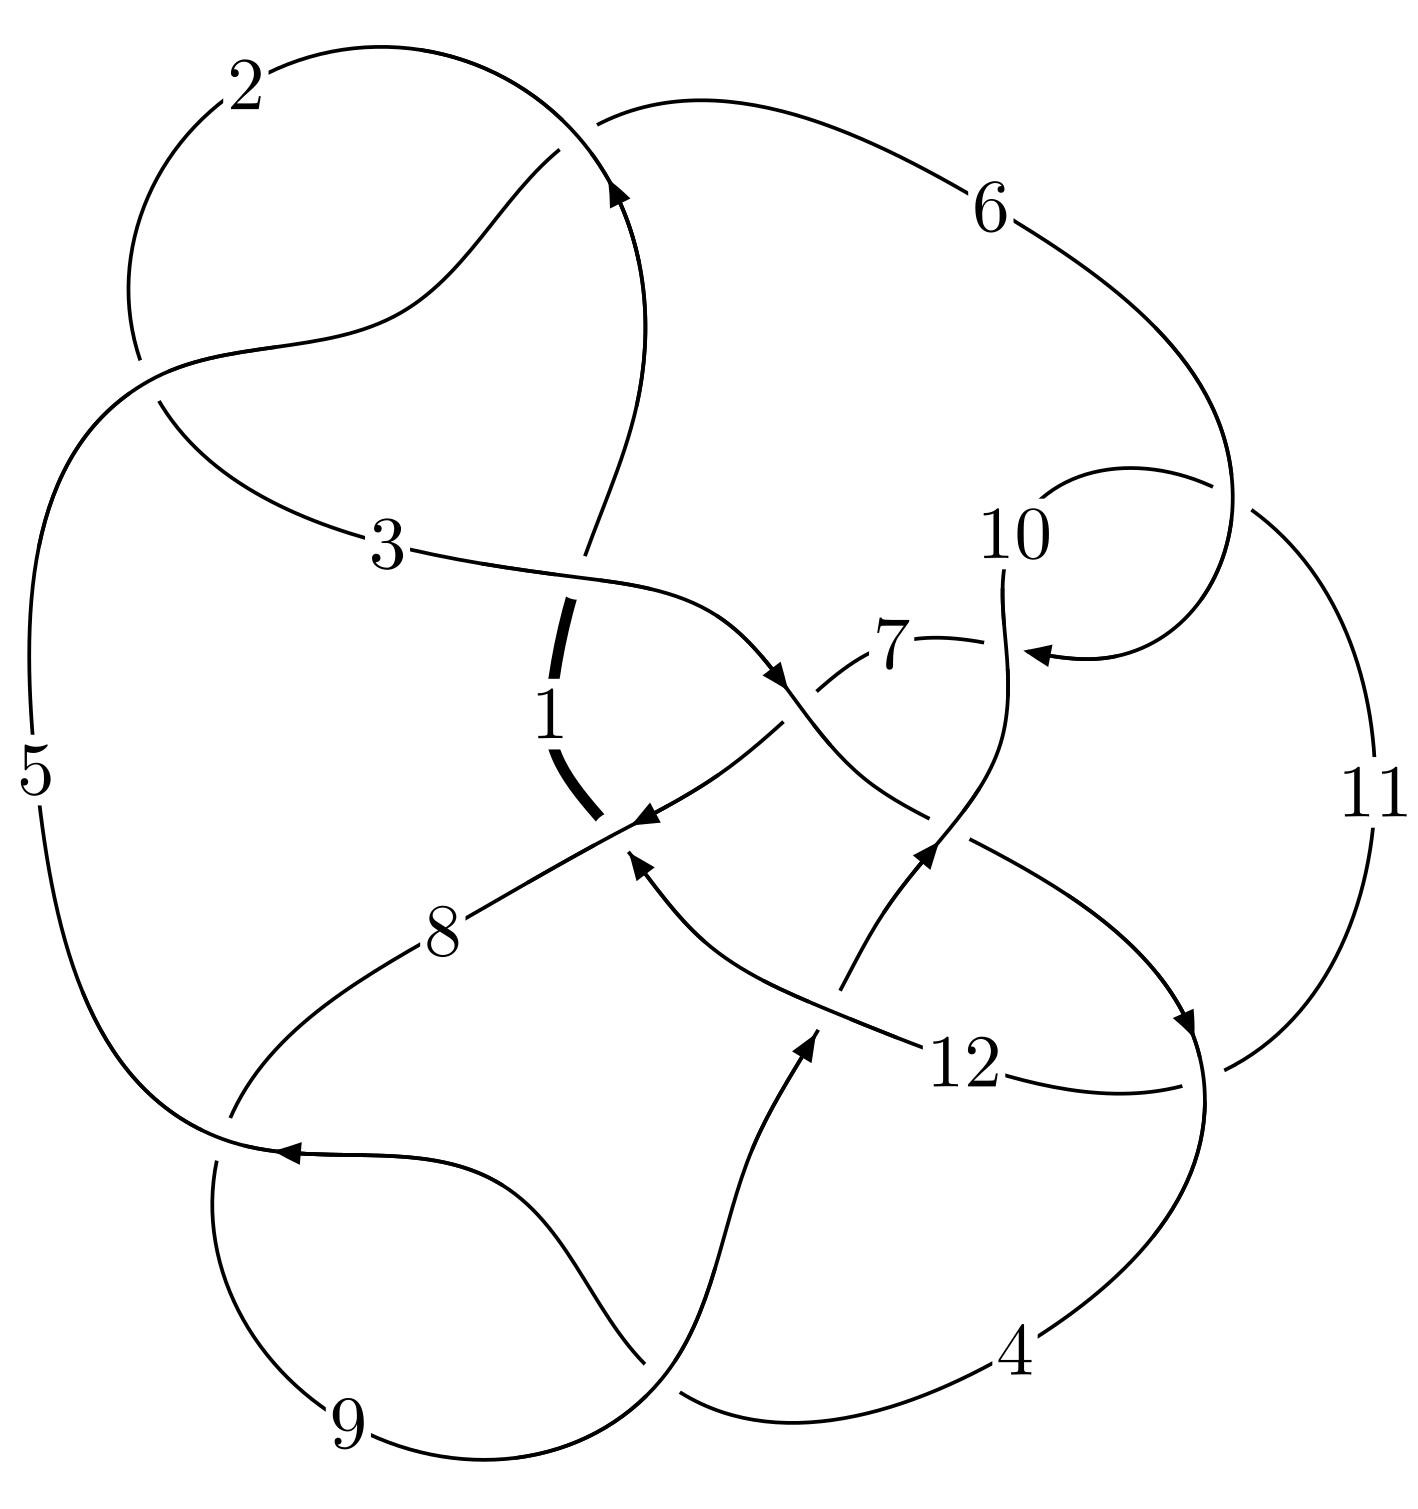
\includegraphics[width=112pt]{../../../GIT/diagram.site/Diagrams/png/2519_12n_0430.png}\\
\ \ \ A knot diagram\footnotemark}&
\allowdisplaybreaks
\textbf{Linearized knot diagam} \\
\cline{2-2}
 &
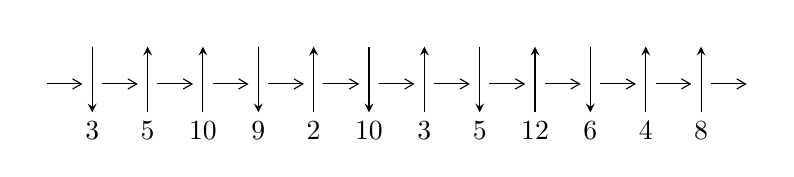
\begin{tikzpicture}[x=20pt, y=17pt]
	% nodes
	\node (C0) at (0, 0) {};
	\node (C1) at (1, 0) {};
	\node (C1U) at (1, +1) {};
	\node (C1D) at (1, -1) {3};

	\node (C2) at (2, 0) {};
	\node (C2U) at (2, +1) {};
	\node (C2D) at (2, -1) {5};

	\node (C3) at (3, 0) {};
	\node (C3U) at (3, +1) {};
	\node (C3D) at (3, -1) {10};

	\node (C4) at (4, 0) {};
	\node (C4U) at (4, +1) {};
	\node (C4D) at (4, -1) {9};

	\node (C5) at (5, 0) {};
	\node (C5U) at (5, +1) {};
	\node (C5D) at (5, -1) {2};

	\node (C6) at (6, 0) {};
	\node (C6U) at (6, +1) {};
	\node (C6D) at (6, -1) {10};

	\node (C7) at (7, 0) {};
	\node (C7U) at (7, +1) {};
	\node (C7D) at (7, -1) {3};

	\node (C8) at (8, 0) {};
	\node (C8U) at (8, +1) {};
	\node (C8D) at (8, -1) {5};

	\node (C9) at (9, 0) {};
	\node (C9U) at (9, +1) {};
	\node (C9D) at (9, -1) {12};

	\node (C10) at (10, 0) {};
	\node (C10U) at (10, +1) {};
	\node (C10D) at (10, -1) {6};

	\node (C11) at (11, 0) {};
	\node (C11U) at (11, +1) {};
	\node (C11D) at (11, -1) {4};

	\node (C12) at (12, 0) {};
	\node (C12U) at (12, +1) {};
	\node (C12D) at (12, -1) {8};
	\node (C13) at (13, 0) {};

	% arrows
	\draw[->,>={angle 60}]
	(C0) edge (C1) (C1) edge (C2) (C2) edge (C3) (C3) edge (C4) (C4) edge (C5) (C5) edge (C6) (C6) edge (C7) (C7) edge (C8) (C8) edge (C9) (C9) edge (C10) (C10) edge (C11) (C11) edge (C12) (C12) edge (C13) ;	\draw[->,>=stealth]
	(C1U) edge (C1D) (C2D) edge (C2U) (C3D) edge (C3U) (C4U) edge (C4D) (C5D) edge (C5U) (C6U) edge (C6D) (C7D) edge (C7U) (C8U) edge (C8D) (C9D) edge (C9U) (C10U) edge (C10D) (C11D) edge (C11U) (C12D) edge (C12U) ;
	\end{tikzpicture} \\
\hhline{~~} \\& 
\textbf{Solving Sequence} \\ \cline{2-2} 
 &
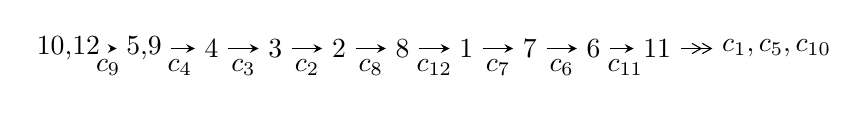
\begin{tikzpicture}[x=23pt, y=7pt]
	% node
	\node (A0) at (-1/8, 0) {10,12};
	\node (A1) at (17/16, 0) {5,9};
	\node (A2) at (17/8, 0) {4};
	\node (A3) at (25/8, 0) {3};
	\node (A4) at (33/8, 0) {2};
	\node (A5) at (41/8, 0) {8};
	\node (A6) at (49/8, 0) {1};
	\node (A7) at (57/8, 0) {7};
	\node (A8) at (65/8, 0) {6};
	\node (A9) at (73/8, 0) {11};
	\node (C1) at (1/2, -1) {$c_{9}$};
	\node (C2) at (13/8, -1) {$c_{4}$};
	\node (C3) at (21/8, -1) {$c_{3}$};
	\node (C4) at (29/8, -1) {$c_{2}$};
	\node (C5) at (37/8, -1) {$c_{8}$};
	\node (C6) at (45/8, -1) {$c_{12}$};
	\node (C7) at (53/8, -1) {$c_{7}$};
	\node (C8) at (61/8, -1) {$c_{6}$};
	\node (C9) at (69/8, -1) {$c_{11}$};
	\node (A10) at (11, 0) {$c_{1},c_{5},c_{10}$};

	% edge
	\draw[->,>=stealth]	
	(A0) edge (A1) (A1) edge (A2) (A2) edge (A3) (A3) edge (A4) (A4) edge (A5) (A5) edge (A6) (A6) edge (A7) (A7) edge (A8) (A8) edge (A9) ;
	\draw[->>,>={angle 60}]	
	(A9) edge (A10);
\end{tikzpicture} \\ 

\end{tabular} \\

\footnotetext{
The image of knot diagram is generated by the software ``\textbf{Draw programme}" developed by Andrew Bartholomew(\url{http://www.layer8.co.uk/maths/draw/index.htm\#Running-draw}), where we modified some parts for our purpose(\url{https://github.com/CATsTAILs/LinksPainter}).
}\phantom \\ \newline 
\centering \textbf{Ideals for irreducible components\footnotemark of $X_{\text{par}}$} 
 
\begin{align*}
I^u_{1}&=\langle 
5393 u^{16}+7516 u^{15}+\cdots+113834 b+14038,\;-56628 u^{16}+74607 u^{15}+\cdots+56917 a+70450,\\
\phantom{I^u_{1}}&\phantom{= \langle  }u^{17}-2 u^{16}+\cdots-3 u+1\rangle \\
I^u_{2}&=\langle 
586 u^{16}+3093 u^{15}+\cdots+176 b+851,\;174 u^{16}+1095 u^{15}+\cdots+88 a+969,\;u^{17}+6 u^{16}+\cdots+7 u+1\rangle \\
\\
\end{align*}
\raggedright * 2 irreducible components of $\dim_{\mathbb{C}}=0$, with total 34 representations.\\
\footnotetext{All coefficients of polynomials are rational numbers. But the coefficients are sometimes approximated in decimal forms when there is not enough margin.}
\newpage
\renewcommand{\arraystretch}{1}
\centering \section*{I. $I^u_{1}= \langle 5393 u^{16}+7516 u^{15}+\cdots+113834 b+14038,\;-56628 u^{16}+74607 u^{15}+\cdots+56917 a+70450,\;u^{17}-2 u^{16}+\cdots-3 u+1 \rangle$}
\flushleft \textbf{(i) Arc colorings}\\
\begin{tabular}{m{7pt} m{180pt} m{7pt} m{180pt} }
\flushright $a_{10}=$&$\begin{pmatrix}1\\0\end{pmatrix}$ \\
\flushright $a_{12}=$&$\begin{pmatrix}0\\u\end{pmatrix}$ \\
\flushright $a_{5}=$&$\begin{pmatrix}0.994922 u^{16}-1.31080 u^{15}+\cdots+4.13788 u-1.23777\\-0.0473760 u^{16}-0.0660260 u^{15}+\cdots+0.122169 u-0.123320\end{pmatrix}$ \\
\flushright $a_{9}=$&$\begin{pmatrix}1\\u^2\end{pmatrix}$ \\
\flushright $a_{4}=$&$\begin{pmatrix}0.477898 u^{16}-0.823497 u^{15}+\cdots+3.21785 u-0.682046\\-0.443259 u^{16}+0.608096 u^{15}+\cdots-1.00104 u+0.423424\end{pmatrix}$ \\
\flushright $a_{3}=$&$\begin{pmatrix}0.921157 u^{16}-1.43159 u^{15}+\cdots+4.21889 u-1.10547\\-0.443259 u^{16}+0.608096 u^{15}+\cdots-1.00104 u+0.423424\end{pmatrix}$ \\
\flushright $a_{2}=$&$\begin{pmatrix}-0.425585 u^{16}+0.0861869 u^{15}+\cdots+1.60377 u+0.623056\\- u^2\end{pmatrix}$ \\
\flushright $a_{8}=$&$\begin{pmatrix}0.328742 u^{16}-1.22857 u^{15}+\cdots+1.16794 u-1.55584\\-0.0276279 u^{16}+0.220628 u^{15}+\cdots-0.602685 u+0.647443\end{pmatrix}$ \\
\flushright $a_{1}=$&$\begin{pmatrix}-0.112286 u^{16}+0.00399705 u^{15}+\cdots+2.05786 u-0.526196\\0.290282 u^{16}-0.397597 u^{15}+\cdots+0.452817 u+0.188204\end{pmatrix}$ \\
\flushright $a_{7}=$&$\begin{pmatrix}-2.03864 u^{16}+3.21241 u^{15}+\cdots-6.13918 u+2.03644\\0.405714 u^{16}-0.285214 u^{15}+\cdots+0.00505121 u+0.301114\end{pmatrix}$ \\
\flushright $a_{6}=$&$\begin{pmatrix}-1.63293 u^{16}+2.92720 u^{15}+\cdots-6.13413 u+2.33755\\0.405714 u^{16}-0.285214 u^{15}+\cdots+0.00505121 u+0.301114\end{pmatrix}$ \\
\flushright $a_{11}=$&$\begin{pmatrix}-1.71543 u^{16}+2.52797 u^{15}+\cdots-3.79178 u+2.31009\\-0.0167876 u^{16}+0.211167 u^{15}+\cdots-0.0891034 u+0.108351\end{pmatrix}$\\&\end{tabular}
\flushleft \textbf{(ii) Obstruction class $= -1$}\\~\\
\flushleft \textbf{(iii) Cusp Shapes $= -\frac{49715}{8131} u^{16}+\frac{80546}{8131} u^{15}+\cdots-\frac{140656}{8131} u+\frac{65802}{8131}$}\\~\\
\newpage\renewcommand{\arraystretch}{1}
\flushleft \textbf{(iv) u-Polynomials at the component}\newline \\
\begin{tabular}{m{50pt}|m{274pt}}
Crossings & \hspace{64pt}u-Polynomials at each crossing \\
\hline $$\begin{aligned}c_{1}\end{aligned}$$&$\begin{aligned}
&u^{17}+31 u^{16}+\cdots-143264 u-13456
\end{aligned}$\\
\hline $$\begin{aligned}c_{2},c_{5}\end{aligned}$$&$\begin{aligned}
&u^{17}+5 u^{16}+\cdots+324 u-116
\end{aligned}$\\
\hline $$\begin{aligned}c_{3}\end{aligned}$$&$\begin{aligned}
&u^{17}-8 u^{15}+\cdots-353 u-89
\end{aligned}$\\
\hline $$\begin{aligned}c_{4},c_{8}\end{aligned}$$&$\begin{aligned}
&u^{17}+14 u^{15}+\cdots+664 u-161
\end{aligned}$\\
\hline $$\begin{aligned}c_{6},c_{10}\end{aligned}$$&$\begin{aligned}
&u^{17}-13 u^{15}+\cdots+491 u-113
\end{aligned}$\\
\hline $$\begin{aligned}c_{7}\end{aligned}$$&$\begin{aligned}
&u^{17}+3 u^{16}+\cdots-2 u-1
\end{aligned}$\\
\hline $$\begin{aligned}c_{9}\end{aligned}$$&$\begin{aligned}
&u^{17}+2 u^{16}+\cdots-3 u-1
\end{aligned}$\\
\hline $$\begin{aligned}c_{11}\end{aligned}$$&$\begin{aligned}
&u^{17}-2 u^{16}+\cdots-7040 u-5641
\end{aligned}$\\
\hline $$\begin{aligned}c_{12}\end{aligned}$$&$\begin{aligned}
&u^{17}-4 u^{16}+\cdots+54780 u-10369
\end{aligned}$\\
\hline
\end{tabular}\\~\\
\newpage\renewcommand{\arraystretch}{1}
\flushleft \textbf{(v) Riley Polynomials at the component}\newline \\
\begin{tabular}{m{50pt}|m{274pt}}
Crossings & \hspace{64pt}Riley Polynomials at each crossing \\
\hline $$\begin{aligned}c_{1}\end{aligned}$$&$\begin{aligned}
&y^{17}+11 y^{16}+\cdots+7175468160 y-181063936
\end{aligned}$\\
\hline $$\begin{aligned}c_{2},c_{5}\end{aligned}$$&$\begin{aligned}
&y^{17}+31 y^{16}+\cdots-143264 y-13456
\end{aligned}$\\
\hline $$\begin{aligned}c_{3}\end{aligned}$$&$\begin{aligned}
&y^{17}-16 y^{16}+\cdots+32227 y-7921
\end{aligned}$\\
\hline $$\begin{aligned}c_{4},c_{8}\end{aligned}$$&$\begin{aligned}
&y^{17}+28 y^{16}+\cdots+580966 y-25921
\end{aligned}$\\
\hline $$\begin{aligned}c_{6},c_{10}\end{aligned}$$&$\begin{aligned}
&y^{17}-26 y^{16}+\cdots+68417 y-12769
\end{aligned}$\\
\hline $$\begin{aligned}c_{7}\end{aligned}$$&$\begin{aligned}
&y^{17}+31 y^{16}+\cdots-2 y-1
\end{aligned}$\\
\hline $$\begin{aligned}c_{9}\end{aligned}$$&$\begin{aligned}
&y^{17}+2 y^{16}+\cdots+y-1
\end{aligned}$\\
\hline $$\begin{aligned}c_{11}\end{aligned}$$&$\begin{aligned}
&y^{17}-28 y^{16}+\cdots+15817138 y-31820881
\end{aligned}$\\
\hline $$\begin{aligned}c_{12}\end{aligned}$$&$\begin{aligned}
&y^{17}+40 y^{16}+\cdots-105102598 y-107516161
\end{aligned}$\\
\hline
\end{tabular}\\~\\
\newpage\flushleft \textbf{(vi) Complex Volumes and Cusp Shapes}
$$\begin{array}{c|c|c}  
\text{Solutions to }I^u_{1}& \I (\text{vol} + \sqrt{-1}CS) & \text{Cusp shape}\\
 \hline 
\begin{aligned}
u &= \phantom{-}0.362254 + 0.899149 I \\
a &= \phantom{-}0.508122 - 0.988405 I \\
b &= -0.494404 + 0.009659 I\end{aligned}
 & -7.23529 - 1.23787 I & \phantom{-}0.881318 - 0.776121 I \\ \hline\begin{aligned}
u &= \phantom{-}0.362254 - 0.899149 I \\
a &= \phantom{-}0.508122 + 0.988405 I \\
b &= -0.494404 - 0.009659 I\end{aligned}
 & -7.23529 + 1.23787 I & \phantom{-}0.881318 + 0.776121 I \\ \hline\begin{aligned}
u &= \phantom{-}0.521342 + 0.748526 I \\
a &= -0.957661 - 0.986783 I \\
b &= \phantom{-}0.120151 + 0.418864 I\end{aligned}
 & -6.57952 + 4.86431 I & -3.62543 - 7.86944 I \\ \hline\begin{aligned}
u &= \phantom{-}0.521342 - 0.748526 I \\
a &= -0.957661 + 0.986783 I \\
b &= \phantom{-}0.120151 - 0.418864 I\end{aligned}
 & -6.57952 - 4.86431 I & -3.62543 + 7.86944 I \\ \hline\begin{aligned}
u &= -0.179836 + 0.612795 I \\
a &= \phantom{-}0.209052 + 0.316220 I \\
b &= \phantom{-}0.642189 + 0.262178 I\end{aligned}
 & -0.94259 - 1.35597 I & -2.95073 + 4.86153 I \\ \hline\begin{aligned}
u &= -0.179836 - 0.612795 I \\
a &= \phantom{-}0.209052 - 0.316220 I \\
b &= \phantom{-}0.642189 - 0.262178 I\end{aligned}
 & -0.94259 + 1.35597 I & -2.95073 - 4.86153 I \\ \hline\begin{aligned}
u &= -0.608474\phantom{ +0.000000I} \\
a &= -1.54897\phantom{ +0.000000I} \\
b &= -0.776291\phantom{ +0.000000I}\end{aligned}
 & \phantom{-}1.24807\phantom{ +0.000000I} & \phantom{-}10.3340\phantom{ +0.000000I} \\ \hline\begin{aligned}
u &= -1.103650 + 0.854632 I \\
a &= -0.354799 + 1.315260 I \\
b &= \phantom{-}1.46583 - 0.63451 I\end{aligned}
 & \phantom{-}2.93182 - 3.02594 I & \phantom{-}2.01363 + 1.83200 I \\ \hline\begin{aligned}
u &= -1.103650 - 0.854632 I \\
a &= -0.354799 - 1.315260 I \\
b &= \phantom{-}1.46583 + 0.63451 I\end{aligned}
 & \phantom{-}2.93182 + 3.02594 I & \phantom{-}2.01363 - 1.83200 I \\ \hline\begin{aligned}
u &= -0.86904 + 1.16197 I \\
a &= \phantom{-}1.202500 - 0.252987 I \\
b &= -1.63818 - 0.34892 I\end{aligned}
 & \phantom{-}1.82701 - 4.29273 I & \phantom{-}1.50320 + 2.40550 I\\
 \hline 
 \end{array}$$\newpage$$\begin{array}{c|c|c}  
\text{Solutions to }I^u_{1}& \I (\text{vol} + \sqrt{-1}CS) & \text{Cusp shape}\\
 \hline 
\begin{aligned}
u &= -0.86904 - 1.16197 I \\
a &= \phantom{-}1.202500 + 0.252987 I \\
b &= -1.63818 + 0.34892 I\end{aligned}
 & \phantom{-}1.82701 + 4.29273 I & \phantom{-}1.50320 - 2.40550 I \\ \hline\begin{aligned}
u &= \phantom{-}1.00617 + 1.09412 I \\
a &= \phantom{-}0.91587 + 1.51470 I \\
b &= -2.31303 - 0.28490 I\end{aligned}
 & \phantom{-}17.3067 + 11.4081 I & \phantom{-}1.65806 - 4.29006 I \\ \hline\begin{aligned}
u &= \phantom{-}1.00617 - 1.09412 I \\
a &= \phantom{-}0.91587 - 1.51470 I \\
b &= -2.31303 + 0.28490 I\end{aligned}
 & \phantom{-}17.3067 - 11.4081 I & \phantom{-}1.65806 + 4.29006 I \\ \hline\begin{aligned}
u &= \phantom{-}1.11198 + 0.98896 I \\
a &= -0.990744 - 0.722226 I \\
b &= \phantom{-}2.32313 - 0.15197 I\end{aligned}
 & \phantom{-}17.7203 - 3.6735 I & \phantom{-}1.99465 + 0.48580 I \\ \hline\begin{aligned}
u &= \phantom{-}1.11198 - 0.98896 I \\
a &= -0.990744 + 0.722226 I \\
b &= \phantom{-}2.32313 + 0.15197 I\end{aligned}
 & \phantom{-}17.7203 + 3.6735 I & \phantom{-}1.99465 - 0.48580 I \\ \hline\begin{aligned}
u &= \phantom{-}0.455022 + 0.222930 I \\
a &= \phantom{-}0.24214 + 2.49180 I \\
b &= -0.217538 - 0.475765 I\end{aligned}
 & \phantom{-}0.66649 + 1.83609 I & \phantom{-}2.85826 - 4.77361 I \\ \hline\begin{aligned}
u &= \phantom{-}0.455022 - 0.222930 I \\
a &= \phantom{-}0.24214 - 2.49180 I \\
b &= -0.217538 + 0.475765 I\end{aligned}
 & \phantom{-}0.66649 - 1.83609 I & \phantom{-}2.85826 + 4.77361 I\\
 \hline 
 \end{array}$$\newpage\newpage\renewcommand{\arraystretch}{1}
\centering \section*{II. $I^u_{2}= \langle 586 u^{16}+3093 u^{15}+\cdots+176 b+851,\;174 u^{16}+1095 u^{15}+\cdots+88 a+969,\;u^{17}+6 u^{16}+\cdots+7 u+1 \rangle$}
\flushleft \textbf{(i) Arc colorings}\\
\begin{tabular}{m{7pt} m{180pt} m{7pt} m{180pt} }
\flushright $a_{10}=$&$\begin{pmatrix}1\\0\end{pmatrix}$ \\
\flushright $a_{12}=$&$\begin{pmatrix}0\\u\end{pmatrix}$ \\
\flushright $a_{5}=$&$\begin{pmatrix}-1.97727 u^{16}-12.4432 u^{15}+\cdots-40.8977 u-11.0114\\-3.32955 u^{16}-17.5739 u^{15}+\cdots-22.4830 u-4.83523\end{pmatrix}$ \\
\flushright $a_{9}=$&$\begin{pmatrix}1\\u^2\end{pmatrix}$ \\
\flushright $a_{4}=$&$\begin{pmatrix}-5.89773 u^{16}-33.6193 u^{15}+\cdots-69.4148 u-16.4261\\-4.01136 u^{16}-22.0909 u^{15}+\cdots-34.9886 u-7.18182\end{pmatrix}$ \\
\flushright $a_{3}=$&$\begin{pmatrix}-1.88636 u^{16}-11.5284 u^{15}+\cdots-34.4261 u-9.24432\\-4.01136 u^{16}-22.0909 u^{15}+\cdots-34.9886 u-7.18182\end{pmatrix}$ \\
\flushright $a_{2}=$&$\begin{pmatrix}-6.55114 u^{16}-36.0341 u^{15}+\cdots-48.8239 u-7.19318\\- u^2\end{pmatrix}$ \\
\flushright $a_{8}=$&$\begin{pmatrix}0.801136 u^{16}+5.65909 u^{15}+\cdots+7.44886 u-1.43182\\-2.50568 u^{16}-14.9830 u^{15}+\cdots-33.8068 u-7.65341\end{pmatrix}$ \\
\flushright $a_{1}=$&$\begin{pmatrix}-5.09659 u^{16}-27.8977 u^{15}+\cdots-40.7784 u-8.42045\\3.01136 u^{16}+16.0909 u^{15}+\cdots+14.9886 u+0.181818\end{pmatrix}$ \\
\flushright $a_{7}=$&$\begin{pmatrix}-3.06818 u^{16}-15.2330 u^{15}+\cdots-9.99432 u-2.90341\\-0.903409 u^{16}-3.97727 u^{15}+\cdots-2.84659 u-1.70455\end{pmatrix}$ \\
\flushright $a_{6}=$&$\begin{pmatrix}-3.97159 u^{16}-19.2102 u^{15}+\cdots-12.8409 u-4.60795\\-0.903409 u^{16}-3.97727 u^{15}+\cdots-2.84659 u-1.70455\end{pmatrix}$ \\
\flushright $a_{11}=$&$\begin{pmatrix}6.00568 u^{16}+32.2955 u^{15}+\cdots+54.2443 u+14.8409\\0.704545 u^{16}+3.32386 u^{15}+\cdots+7.35795 u+3.08523\end{pmatrix}$\\&\end{tabular}
\flushleft \textbf{(ii) Obstruction class $= 1$}\\~\\
\flushleft \textbf{(iii) Cusp Shapes $= \frac{71}{88} u^{16}+\frac{87}{22} u^{15}+\cdots-\frac{27}{88} u-\frac{13}{22}$}\\~\\
\newpage\renewcommand{\arraystretch}{1}
\flushleft \textbf{(iv) u-Polynomials at the component}\newline \\
\begin{tabular}{m{50pt}|m{274pt}}
Crossings & \hspace{64pt}u-Polynomials at each crossing \\
\hline $$\begin{aligned}c_{1}\end{aligned}$$&$\begin{aligned}
&u^{17}-15 u^{16}+\cdots-144 u+16
\end{aligned}$\\
\hline $$\begin{aligned}c_{2}\end{aligned}$$&$\begin{aligned}
&u^{17}+3 u^{16}+\cdots+8 u+4
\end{aligned}$\\
\hline $$\begin{aligned}c_{3}\end{aligned}$$&$\begin{aligned}
&u^{17}+2 u^{15}+\cdots- u-1
\end{aligned}$\\
\hline $$\begin{aligned}c_{4}\end{aligned}$$&$\begin{aligned}
&u^{17}+6 u^{15}+\cdots+2 u-1
\end{aligned}$\\
\hline $$\begin{aligned}c_{5}\end{aligned}$$&$\begin{aligned}
&u^{17}-3 u^{16}+\cdots+8 u-4
\end{aligned}$\\
\hline $$\begin{aligned}c_{6}\end{aligned}$$&$\begin{aligned}
&u^{17}-2 u^{16}+\cdots+3 u-1
\end{aligned}$\\
\hline $$\begin{aligned}c_{7}\end{aligned}$$&$\begin{aligned}
&u^{17}+u^{16}+\cdots+2 u+1
\end{aligned}$\\
\hline $$\begin{aligned}c_{8}\end{aligned}$$&$\begin{aligned}
&u^{17}+6 u^{15}+\cdots+2 u+1
\end{aligned}$\\
\hline $$\begin{aligned}c_{9}\end{aligned}$$&$\begin{aligned}
&u^{17}+6 u^{16}+\cdots+7 u+1
\end{aligned}$\\
\hline $$\begin{aligned}c_{10}\end{aligned}$$&$\begin{aligned}
&u^{17}+2 u^{16}+\cdots+3 u+1
\end{aligned}$\\
\hline $$\begin{aligned}c_{11}\end{aligned}$$&$\begin{aligned}
&u^{17}-6 u^{15}+\cdots-2 u+1
\end{aligned}$\\
\hline $$\begin{aligned}c_{12}\end{aligned}$$&$\begin{aligned}
&u^{17}+2 u^{16}+\cdots-6 u+1
\end{aligned}$\\
\hline
\end{tabular}\\~\\
\newpage\renewcommand{\arraystretch}{1}
\flushleft \textbf{(v) Riley Polynomials at the component}\newline \\
\begin{tabular}{m{50pt}|m{274pt}}
Crossings & \hspace{64pt}Riley Polynomials at each crossing \\
\hline $$\begin{aligned}c_{1}\end{aligned}$$&$\begin{aligned}
&y^{17}-21 y^{16}+\cdots+896 y-256
\end{aligned}$\\
\hline $$\begin{aligned}c_{2},c_{5}\end{aligned}$$&$\begin{aligned}
&y^{17}+15 y^{16}+\cdots-144 y-16
\end{aligned}$\\
\hline $$\begin{aligned}c_{3}\end{aligned}$$&$\begin{aligned}
&y^{17}+4 y^{16}+\cdots+7 y-1
\end{aligned}$\\
\hline $$\begin{aligned}c_{4},c_{8}\end{aligned}$$&$\begin{aligned}
&y^{17}+12 y^{16}+\cdots-14 y-1
\end{aligned}$\\
\hline $$\begin{aligned}c_{6},c_{10}\end{aligned}$$&$\begin{aligned}
&y^{17}-6 y^{16}+\cdots-3 y-1
\end{aligned}$\\
\hline $$\begin{aligned}c_{7}\end{aligned}$$&$\begin{aligned}
&y^{17}+31 y^{16}+\cdots+46 y-1
\end{aligned}$\\
\hline $$\begin{aligned}c_{9}\end{aligned}$$&$\begin{aligned}
&y^{17}+2 y^{16}+\cdots+9 y-1
\end{aligned}$\\
\hline $$\begin{aligned}c_{11}\end{aligned}$$&$\begin{aligned}
&y^{17}-12 y^{16}+\cdots-22 y-1
\end{aligned}$\\
\hline $$\begin{aligned}c_{12}\end{aligned}$$&$\begin{aligned}
&y^{17}+8 y^{16}+\cdots+30 y-1
\end{aligned}$\\
\hline
\end{tabular}\\~\\
\newpage\flushleft \textbf{(vi) Complex Volumes and Cusp Shapes}
$$\begin{array}{c|c|c}  
\text{Solutions to }I^u_{2}& \I (\text{vol} + \sqrt{-1}CS) & \text{Cusp shape}\\
 \hline 
\begin{aligned}
u &= -0.663834 + 0.651775 I \\
a &= \phantom{-}0.943799 - 0.890365 I \\
b &= -1.067980 - 0.354608 I\end{aligned}
 & \phantom{-}1.273240 - 0.057282 I & \phantom{-}2.81611 - 0.19040 I \\ \hline\begin{aligned}
u &= -0.663834 - 0.651775 I \\
a &= \phantom{-}0.943799 + 0.890365 I \\
b &= -1.067980 + 0.354608 I\end{aligned}
 & \phantom{-}1.273240 + 0.057282 I & \phantom{-}2.81611 + 0.19040 I \\ \hline\begin{aligned}
u &= \phantom{-}0.833502 + 0.399060 I \\
a &= -0.031669 + 0.929376 I \\
b &= -0.809508 - 0.849987 I\end{aligned}
 & -2.84392 + 1.35053 I & \phantom{-}2.24307 - 2.14121 I \\ \hline\begin{aligned}
u &= \phantom{-}0.833502 - 0.399060 I \\
a &= -0.031669 - 0.929376 I \\
b &= -0.809508 + 0.849987 I\end{aligned}
 & -2.84392 - 1.35053 I & \phantom{-}2.24307 + 2.14121 I \\ \hline\begin{aligned}
u &= \phantom{-}0.532887 + 0.962901 I \\
a &= -1.44876 - 0.06054 I \\
b &= \phantom{-}0.748089 - 0.622928 I\end{aligned}
 & -4.72942 + 3.29248 I & \phantom{-}0.14195 - 3.24278 I \\ \hline\begin{aligned}
u &= \phantom{-}0.532887 - 0.962901 I \\
a &= -1.44876 + 0.06054 I \\
b &= \phantom{-}0.748089 + 0.622928 I\end{aligned}
 & -4.72942 - 3.29248 I & \phantom{-}0.14195 + 3.24278 I \\ \hline\begin{aligned}
u &= -0.042338 + 0.877922 I \\
a &= -0.23026 - 1.50709 I \\
b &= \phantom{-}0.611186 + 0.415473 I\end{aligned}
 & -8.17306 + 1.94502 I & -5.85947 - 3.89574 I \\ \hline\begin{aligned}
u &= -0.042338 - 0.877922 I \\
a &= -0.23026 + 1.50709 I \\
b &= \phantom{-}0.611186 - 0.415473 I\end{aligned}
 & -8.17306 - 1.94502 I & -5.85947 + 3.89574 I \\ \hline\begin{aligned}
u &= -0.660026 + 1.092400 I \\
a &= -0.184327 + 0.822457 I \\
b &= \phantom{-}1.27739 - 0.92461 I\end{aligned}
 & -0.14701 - 5.07773 I & -2.20879 + 6.02432 I \\ \hline\begin{aligned}
u &= -0.660026 - 1.092400 I \\
a &= -0.184327 - 0.822457 I \\
b &= \phantom{-}1.27739 + 0.92461 I\end{aligned}
 & -0.14701 + 5.07773 I & -2.20879 - 6.02432 I\\
 \hline 
 \end{array}$$\newpage$$\begin{array}{c|c|c}  
\text{Solutions to }I^u_{2}& \I (\text{vol} + \sqrt{-1}CS) & \text{Cusp shape}\\
 \hline 
\begin{aligned}
u &= -0.559508 + 0.431950 I \\
a &= \phantom{-}0.51799 - 1.76316 I \\
b &= \phantom{-}0.215995 + 0.599967 I\end{aligned}
 & -6.21673 - 4.10194 I & \phantom{-}1.014362 - 0.459850 I \\ \hline\begin{aligned}
u &= -0.559508 - 0.431950 I \\
a &= \phantom{-}0.51799 + 1.76316 I \\
b &= \phantom{-}0.215995 - 0.599967 I\end{aligned}
 & -6.21673 + 4.10194 I & \phantom{-}1.014362 + 0.459850 I \\ \hline\begin{aligned}
u &= -1.20705 + 0.84824 I \\
a &= -0.473403 + 1.265630 I \\
b &= \phantom{-}1.95203 + 0.61047 I\end{aligned}
 & \phantom{-}4.35554 - 2.89495 I & \phantom{-}10.74646 + 0.70267 I \\ \hline\begin{aligned}
u &= -1.20705 - 0.84824 I \\
a &= -0.473403 - 1.265630 I \\
b &= \phantom{-}1.95203 - 0.61047 I\end{aligned}
 & \phantom{-}4.35554 + 2.89495 I & \phantom{-}10.74646 - 0.70267 I \\ \hline\begin{aligned}
u &= -1.07765 + 1.20640 I \\
a &= \phantom{-}0.558261 - 1.009500 I \\
b &= -2.68997 + 0.21065 I\end{aligned}
 & \phantom{-}3.26824 - 5.33607 I & \phantom{-}6.67246 + 8.79937 I \\ \hline\begin{aligned}
u &= -1.07765 - 1.20640 I \\
a &= \phantom{-}0.558261 + 1.009500 I \\
b &= -2.68997 - 0.21065 I\end{aligned}
 & \phantom{-}3.26824 + 5.33607 I & \phantom{-}6.67246 - 8.79937 I \\ \hline\begin{aligned}
u &= -0.311963\phantom{ +0.000000I} \\
a &= -3.30327\phantom{ +0.000000I} \\
b &= -1.47445\phantom{ +0.000000I}\end{aligned}
 & \phantom{-}0.107313\phantom{ +0.000000I} & -0.132300\phantom{ +0.000000I}\\
 \hline 
 \end{array}$$\newpage
\newpage\renewcommand{\arraystretch}{1}
\centering \section*{ III. u-Polynomials}
\begin{tabular}{m{50pt}|m{274pt}}
Crossings & \hspace{64pt}u-Polynomials at each crossing \\
\hline $$\begin{aligned}c_{1}\end{aligned}$$&$\begin{aligned}
&(u^{17}-15 u^{16}+\cdots-144 u+16)\\
&\cdot(u^{17}+31 u^{16}+\cdots-143264 u-13456)
\end{aligned}$\\
\hline $$\begin{aligned}c_{2}\end{aligned}$$&$\begin{aligned}
&(u^{17}+3 u^{16}+\cdots+8 u+4)(u^{17}+5 u^{16}+\cdots+324 u-116)
\end{aligned}$\\
\hline $$\begin{aligned}c_{3}\end{aligned}$$&$\begin{aligned}
&(u^{17}-8 u^{15}+\cdots-353 u-89)(u^{17}+2 u^{15}+\cdots- u-1)
\end{aligned}$\\
\hline $$\begin{aligned}c_{4}\end{aligned}$$&$\begin{aligned}
&(u^{17}+6 u^{15}+\cdots+2 u-1)(u^{17}+14 u^{15}+\cdots+664 u-161)
\end{aligned}$\\
\hline $$\begin{aligned}c_{5}\end{aligned}$$&$\begin{aligned}
&(u^{17}-3 u^{16}+\cdots+8 u-4)(u^{17}+5 u^{16}+\cdots+324 u-116)
\end{aligned}$\\
\hline $$\begin{aligned}c_{6}\end{aligned}$$&$\begin{aligned}
&(u^{17}-13 u^{15}+\cdots+491 u-113)(u^{17}-2 u^{16}+\cdots+3 u-1)
\end{aligned}$\\
\hline $$\begin{aligned}c_{7}\end{aligned}$$&$\begin{aligned}
&(u^{17}+u^{16}+\cdots+2 u+1)(u^{17}+3 u^{16}+\cdots-2 u-1)
\end{aligned}$\\
\hline $$\begin{aligned}c_{8}\end{aligned}$$&$\begin{aligned}
&(u^{17}+6 u^{15}+\cdots+2 u+1)(u^{17}+14 u^{15}+\cdots+664 u-161)
\end{aligned}$\\
\hline $$\begin{aligned}c_{9}\end{aligned}$$&$\begin{aligned}
&(u^{17}+2 u^{16}+\cdots-3 u-1)(u^{17}+6 u^{16}+\cdots+7 u+1)
\end{aligned}$\\
\hline $$\begin{aligned}c_{10}\end{aligned}$$&$\begin{aligned}
&(u^{17}-13 u^{15}+\cdots+491 u-113)(u^{17}+2 u^{16}+\cdots+3 u+1)
\end{aligned}$\\
\hline $$\begin{aligned}c_{11}\end{aligned}$$&$\begin{aligned}
&(u^{17}-6 u^{15}+\cdots-2 u+1)(u^{17}-2 u^{16}+\cdots-7040 u-5641)
\end{aligned}$\\
\hline $$\begin{aligned}c_{12}\end{aligned}$$&$\begin{aligned}
&(u^{17}-4 u^{16}+\cdots+54780 u-10369)(u^{17}+2 u^{16}+\cdots-6 u+1)
\end{aligned}$\\
\hline
\end{tabular}\newpage\renewcommand{\arraystretch}{1}
\centering \section*{ IV. Riley Polynomials}
\begin{tabular}{m{50pt}|m{274pt}}
Crossings & \hspace{64pt}Riley Polynomials at each crossing \\
\hline $$\begin{aligned}c_{1}\end{aligned}$$&$\begin{aligned}
&(y^{17}-21 y^{16}+\cdots+896 y-256)\\
&\cdot(y^{17}+11 y^{16}+\cdots+7175468160 y-181063936)
\end{aligned}$\\
\hline $$\begin{aligned}c_{2},c_{5}\end{aligned}$$&$\begin{aligned}
&(y^{17}+15 y^{16}+\cdots-144 y-16)\\
&\cdot(y^{17}+31 y^{16}+\cdots-143264 y-13456)
\end{aligned}$\\
\hline $$\begin{aligned}c_{3}\end{aligned}$$&$\begin{aligned}
&(y^{17}-16 y^{16}+\cdots+32227 y-7921)(y^{17}+4 y^{16}+\cdots+7 y-1)
\end{aligned}$\\
\hline $$\begin{aligned}c_{4},c_{8}\end{aligned}$$&$\begin{aligned}
&(y^{17}+12 y^{16}+\cdots-14 y-1)(y^{17}+28 y^{16}+\cdots+580966 y-25921)
\end{aligned}$\\
\hline $$\begin{aligned}c_{6},c_{10}\end{aligned}$$&$\begin{aligned}
&(y^{17}-26 y^{16}+\cdots+68417 y-12769)(y^{17}-6 y^{16}+\cdots-3 y-1)
\end{aligned}$\\
\hline $$\begin{aligned}c_{7}\end{aligned}$$&$\begin{aligned}
&(y^{17}+31 y^{16}+\cdots+46 y-1)(y^{17}+31 y^{16}+\cdots-2 y-1)
\end{aligned}$\\
\hline $$\begin{aligned}c_{9}\end{aligned}$$&$\begin{aligned}
&(y^{17}+2 y^{16}+\cdots+9 y-1)(y^{17}+2 y^{16}+\cdots+y-1)
\end{aligned}$\\
\hline $$\begin{aligned}c_{11}\end{aligned}$$&$\begin{aligned}
&(y^{17}-28 y^{16}+\cdots+15817138 y-31820881)\\
&\cdot(y^{17}-12 y^{16}+\cdots-22 y-1)
\end{aligned}$\\
\hline $$\begin{aligned}c_{12}\end{aligned}$$&$\begin{aligned}
&(y^{17}+8 y^{16}+\cdots+30 y-1)\\
&\cdot(y^{17}+40 y^{16}+\cdots-105102598 y-107516161)
\end{aligned}$\\
\hline
\end{tabular}
\vskip 2pc
\end{document}